%%%%%%%%%%%%  Generated using docx2latex.com  %%%%%%%%%%%%%%

%%%%%%%%%%%%  v2.0.0-beta  %%%%%%%%%%%%%%

\documentclass[12pt]{article}
\usepackage{amsmath}
\usepackage{latexsym}
\usepackage{amsfonts}
\usepackage[normalem]{ulem}
\usepackage{soul}
\usepackage{array}
\usepackage{amssymb}
\usepackage{extarrows}
\usepackage{graphicx}
\usepackage[backend=biber,
style=numeric,
sorting=none,
isbn=false,
doi=false,
url=false,
]{biblatex}\addbibresource{bibliography.bib}

\usepackage{subfig}
\usepackage{wrapfig}
\usepackage{txfonts}
\usepackage{wasysym}
\usepackage{enumitem}
\usepackage{adjustbox}
\usepackage{ragged2e}
\usepackage[svgnames,table]{xcolor}
\usepackage{tikz}
\usepackage{longtable}
\usepackage{changepage}
\usepackage{setspace}
\usepackage{hhline}
\usepackage{multicol}
\usepackage{tabto}
\usepackage{float}
\usepackage{multirow}
\usepackage{makecell}
\usepackage{fancyhdr}
\usepackage[toc,page]{appendix}
\usepackage[hidelinks]{hyperref}
\usetikzlibrary{shapes.symbols,shapes.geometric,shadows,arrows.meta}
\tikzset{>={Latex[width=1.5mm,length=2mm]}}
\usepackage{flowchart}\usepackage[paperheight=11.0in,paperwidth=8.5in,left=1.19in,right=1.18in,top=1.04in,bottom=0.19in,headheight=1in]{geometry}
\usepackage[utf8]{inputenc}
\usepackage[T1]{fontenc}
\usepackage[spanish]{babel}
\TabPositions{0.5in,1.0in,1.5in,2.0in,2.5in,3.0in,3.5in,4.0in,4.5in,5.0in,5.5in,6.0in,}

\urlstyle{same}


 %%%%%%%%%%%%  Set Depths for Sections  %%%%%%%%%%%%%%

% 1) Section
% 1.1) SubSection
% 1.1.1) SubSubSection
% 1.1.1.1) Paragraph
% 1.1.1.1.1) Subparagraph


\setcounter{tocdepth}{5}
\setcounter{secnumdepth}{5}


 %%%%%%%%%%%%  Set Depths for Nested Lists created by \begin{enumerate}  %%%%%%%%%%%%%%


\setlistdepth{9}
\renewlist{enumerate}{enumerate}{9}
		\setlist[enumerate,1]{label=\arabic*)}
		\setlist[enumerate,2]{label=\alph*)}
		\setlist[enumerate,3]{label=(\roman*)}
		\setlist[enumerate,4]{label=(\arabic*)}
		\setlist[enumerate,5]{label=(\Alph*)}
		\setlist[enumerate,6]{label=(\Roman*)}
		\setlist[enumerate,7]{label=\arabic*}
		\setlist[enumerate,8]{label=\alph*}
		\setlist[enumerate,9]{label=\roman*}

\renewlist{itemize}{itemize}{9}
		\setlist[itemize]{label=$\cdot$}
		\setlist[itemize,1]{label=\textbullet}
		\setlist[itemize,2]{label=$\circ$}
		\setlist[itemize,3]{label=$\ast$}
		\setlist[itemize,4]{label=$\dagger$}
		\setlist[itemize,5]{label=$\triangleright$}
		\setlist[itemize,6]{label=$\bigstar$}
		\setlist[itemize,7]{label=$\blacklozenge$}
		\setlist[itemize,8]{label=$\prime$}



 %%%%%%%%%%%%  Header here  %%%%%%%%%%%%%%


\pagestyle{fancy}
\fancyhf{}
\chead{ {\fontsize{10pt}{12.0pt}\selectfont  \tabto{1.65in} \uline{Patrones de Diseño de Software\textit{$\bullet$  julio 2020 $\bullet$  \tabto{5.27in}  \tabto{6.03in} }}\par}
\vspace{\baselineskip}
}
\renewcommand{\headrulewidth}{0pt}
\setlength{\topsep}{0pt}\setlength{\parindent}{0pt}
\renewcommand{\arraystretch}{1.3}


%%%%%%%%%%%%%%%%%%%% Document code starts here %%%%%%%%%%%%%%%%%%%%



\begin{document}
\begin{adjustwidth}{0.56in}{0.57in}
\section*{Patrones de Diseño de Software}
\addcontentsline{toc}{section}{Patrones de Diseño de Software}
\end{adjustwidth}

\begin{adjustwidth}{0.56in}{0.57in}
\section*{Belizario Mamani, Loja Mamani, Lizárraga Paolo, Llanque Miguel}
\addcontentsline{toc}{section}{Belizario Mamani, Loja Mamani, Lizárraga Paolo, Llanque Miguel}
\end{adjustwidth}

\begin{adjustwidth}{0.56in}{0.57in}
\section*{July 21, 2020}
\addcontentsline{toc}{section}{July 21, 2020}
\end{adjustwidth}

\begin{adjustwidth}{0.56in}{0.57in}
\subsection*{Abstract}
\addcontentsline{toc}{subsection}{Abstract}
\end{adjustwidth}


\vspace{\baselineskip}
{\fontsize{10pt}{12.0pt}\selectfont There is one thing that is clear:as specific as it is a problem that you are facing during the development of your software, there is a 99$\%$  chance that someone has faced such a similar problem in the past, that it can be model in the same way. \par}\par

{\fontsize{10pt}{12.0pt}\selectfont With modeling we mean that the class structure that makes up the solution to your problem may already have been invented, because you are solving a common problem that other people have already solved before. If the way to solve this problem can be extracted, explained and reused in multiple areas, then we are faced with a software design pattern. \par}\par


\vspace{\baselineskip}

\vspace{\baselineskip}

\vspace{\baselineskip}
\begin{multicols}{2}
\section{Introduccion}
{\fontsize{9pt}{10.8pt}\selectfont En este artículo veremos los patrones de diseño de software que si eres programador seguro que has oído hablar de ellos. Es posible incluso, que ya los estés utilizando en tus aplicaciones. Los patrones de diseño nos ayudan a cumplir muchos principios o reglas de diseño.\par}\par


\vspace{\baselineskip}

\vspace{\baselineskip}
\section{RESUMEN}
{\fontsize{9pt}{10.8pt}\selectfont Hay una cosa que está clara: por muy específico que sea un problema al que te estés enfrentando durante el desarrollo de tu software, hay un 99$\%$  de posibilidades de que alguien se haya enfrentado a un problema tan similar en el pasado, que se pueda modelar de la misma manera. \par}\par


\vspace{\baselineskip}
{\fontsize{9pt}{10.8pt}\selectfont  \par}\par


\vspace{\baselineskip}
{\fontsize{9pt}{10.8pt}\selectfont Con modelado nos referimos a que la estructura de las clases que conforma la solución de tu problema puede estar ya inventada, porque estás resolviendo un problema común que otra gente ya ha solucionado antes. Si la forma de solucionar ese problema se puede extraer, explicar y reutilizar en múltiples ámbitos, entonces nos encontramos ante un patrón de diseño de software\par}\par


\vspace{\baselineskip}
\section{TITULO}

\vspace{\baselineskip}{\fontsize{9pt}{10.8pt}\selectfont \ \ \ \ \ \ \ \ \ \ \ \ \ \ \  Patrones de diseño de software\par}\par

\section{AUTORES}

\vspace{\baselineskip}
{\fontsize{9pt}{10.8pt}\selectfont Los autores de este trabajo final de unidad son:\par}\par


\vspace{\baselineskip}


%%%%%%%%%%%%%%%%%%%% Figure/Image No: 1 starts here %%%%%%%%%%%%%%%%%%%%

\begin{figure}[H]		
\includegraphics[width=1.75in,height=1.44in]{./media/image1.png}
\end{figure}


%%%%%%%%%%%%%%%%%%%% Figure/Image No: 1 Ends here %%%%%%%%%%%%%%%%%%%%

\begin{itemize}
	\item {\fontsize{9pt}{10.8pt}\selectfont Paolo Lizárraga\par}\par


\end{itemize}
\vspace{\baselineskip}

%%%%%%%%%%%%%%%%%%%% Figure/Image No: 2 starts here %%%%%%%%%%%%%%%%%%%%

\begin{figure}[H]		
\includegraphics[width=1.84in,height=1.72in]{./media/image2.png}
\end{figure}


%%%%%%%%%%%%%%%%%%%% Figure/Image No: 2 Ends here %%%%%%%%%%%%%%%%%%%%

\begin{itemize}
	\item {\fontsize{9pt}{10.8pt}\selectfont Anthony Belizario\par}\par


\vspace{\baselineskip}

\vspace{\baselineskip}

\vspace{\baselineskip}
	\item {\fontsize{9pt}{10.8pt}\selectfont Daniel Loja\par}\par



%%%%%%%%%%%%%%%%%%%% Figure/Image No: 3 starts here %%%%%%%%%%%%%%%%%%%%


\begin{figure}[H]	\begin{subfigure}		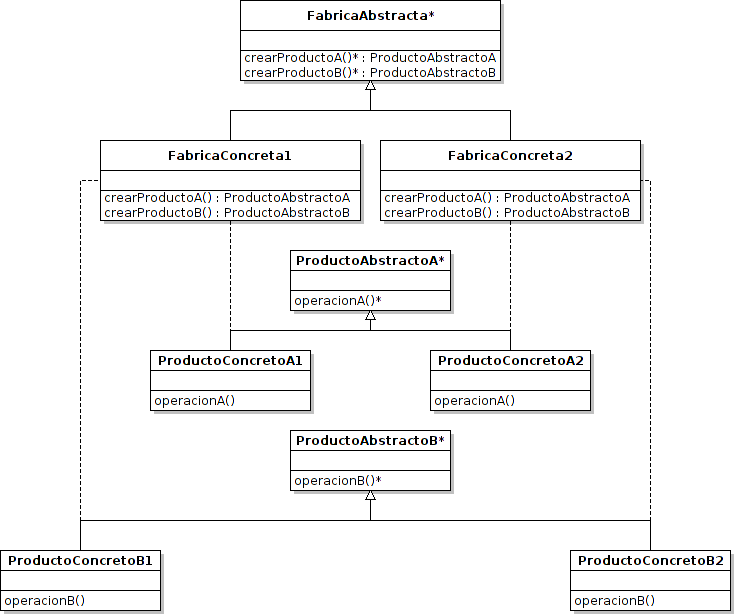
\includegraphics[width=0.45\textwidth]{./media/image3.png}
	\end{subfigure}
~	\begin{subfigure}		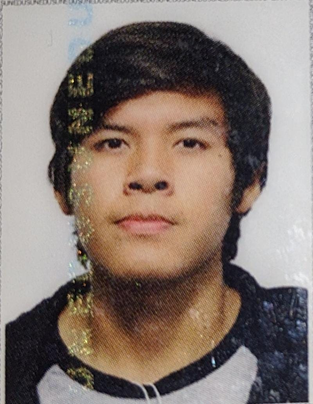
\includegraphics[width=0.45\textwidth]{./media/image4.png}
	\end{subfigure}
~
\end{figure}


%%%%%%%%%%%%%%%%%%%% Figure/Image No: 3 Ends here %%%%%%%%%%%%%%%%%%%%

\par

	\item {\fontsize{9pt}{10.8pt}\selectfont Miguel LLanque\par}
\end{itemize}\par



%%%%%%%%%%%%%%%%%%%% Figure/Image No: 4 starts here %%%%%%%%%%%%%%%%%%%%

\begin{figure}[H]		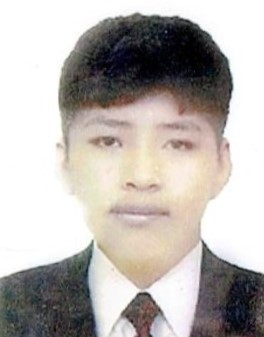
\includegraphics[width=1.68in,height=1.6in]{./media/image5.jpeg}
\end{figure}


%%%%%%%%%%%%%%%%%%%% Figure/Image No: 4 Ends here %%%%%%%%%%%%%%%%%%%%

\par


\vspace{\baselineskip}\section*{ V.DESARROLLO}
\addcontentsline{toc}{section}{ V.DESARROLLO}
\begin{enumerate}
	\item \textbf{Patrones Creacionales}\par

{\fontsize{9pt}{10.8pt}\selectfont Son los que facilitan la tarea de creación de nuevos objetos, de tal forma que el proceso de creación pueda ser desacoplado de la implementación\ del resto del sistema.  \par}\par


\vspace{\baselineskip}
{\fontsize{9pt}{10.8pt}\selectfont Estos\ nos proveen soluciones para la creación de objetos, permitiéndonos hacer un sistema independiente de cómo sus objetos son creados.  \par}\par


\vspace{\baselineskip}
{\fontsize{9pt}{10.8pt}\selectfont Los Patrones creacionales más conocidos:\par}\par


\vspace{\baselineskip}
\begin{itemize}
	\item {\fontsize{9pt}{10.8pt}\selectfont \textbf{Patrón Abstract Factory} \par}\par


\vspace{\baselineskip}


%%%%%%%%%%%%%%%%%%%% Figure/Image No: 5 starts here %%%%%%%%%%%%%%%%%%%%

\begin{figure}[H]		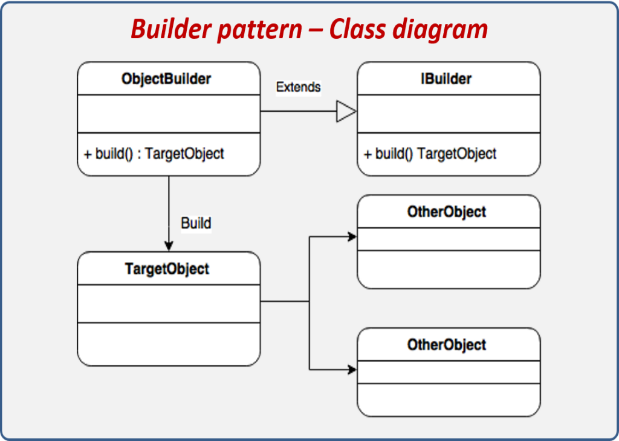
\includegraphics[width=2.81in,height=2.01in]{./media/image6.png}
\end{figure}


%%%%%%%%%%%%%%%%%%%% Figure/Image No: 5 Ends here %%%%%%%%%%%%%%%%%%%%

{\fontsize{9pt}{10.8pt}\selectfont \textbf{Definición:} Es un patrón de diseño para el desarrollo de software. Provee una interfaz para crear familias de objetos relacionados o dependientes entre ellos sin especificar una clase en concreto.\par}\par


\vspace{\baselineskip}
{\fontsize{9pt}{10.8pt}\selectfont Este patrón se puede aplicar cuando: \par}\par

\begin{itemize}
	\item {\fontsize{9pt}{10.8pt}\selectfont Un sistema debe ser independiente de cómo sus objetos son creados. \par}\par

	\item {\fontsize{9pt}{10.8pt}\selectfont Un sistema debe ser ‘configurado’ con una cierta familia de productos. \par}\par

	\item {\fontsize{9pt}{10.8pt}\selectfont Se necesita reforzar la noción de dependencia mutua entre ciertos objetos. \par}
\end{itemize}\par


\vspace{\baselineskip}

\vspace{\baselineskip}

\vspace{\baselineskip}

\vspace{\baselineskip}
{\fontsize{9pt}{10.8pt}\selectfont \textbf{Participantes: }\par}\par


\vspace{\baselineskip}
{\fontsize{9pt}{10.8pt}\selectfont \textbf{Fabrica Abstracta$\ast$ :} Define un conjunto de métodos (interfaz) para la creación de productos abstractos. \par}\par


\vspace{\baselineskip}
{\fontsize{9pt}{10.8pt}\selectfont \textbf{FabricaConcreta1/2:} Implementa la interfaz de la Fabrica Abstracta para la creación de los distintos productos concretos. \par}\par


\vspace{\baselineskip}
{\fontsize{9pt}{10.8pt}\selectfont \textbf{ProductoAbstractoA$\ast$ /B$\ast$ :} Define la interfaz de los objetos de tipo ProductoA/B. \par}\par


\vspace{\baselineskip}
{\fontsize{9pt}{10.8pt}\selectfont \textbf{ProductoConcretoA1/A2/B1/B2}: Implementan su respectiva interfaz representando un producto concreto.\par}\par


\vspace{\baselineskip}
{\fontsize{9pt}{10.8pt}\selectfont   \textbf{$\bullet$ \ \  Patrón Builder}\par}\par

{\fontsize{9pt}{10.8pt}\selectfont \textbf{Definición:} Este es un patrón bastante simple pero muy útil, el cual nos permite crear objetos complejos a través de uno más simple. Es muy común encontrarnos con situaciones en las cuales tenemos que crear objetos compuestos de forma manual y repetidas veces, lo que nos lleva a tener que establecer cada propiedad del objeto y si ésta además tiene objetos compuestos dentro, tenemos que crearlos primero para después ser asignados al objeto que estamos creando. Esto desde luego que se hace una tarea tediosa y cansada, sobre todo cuando tenemos que crear de manera frecuente los objetos.\par}\par


\vspace{\baselineskip}
{\fontsize{9pt}{10.8pt}\selectfont \textbf{Participantes: }\par}\par


\vspace{\baselineskip}
{\fontsize{9pt}{10.8pt}\selectfont \textbf{ObjectBuilder:} Esta es la clase que utilizaremos para crear los TarjetObjet, esta clase debe de heredar de IBuilder e implementar el método build, el cual será utilizado para crear al TarjetObject. Como regla general todos los métodos de esta clase retornan a si mismo con la finalidad de agilizar la creación, esta clase por lo general es creada como una clase interna del TargetObject. \par}\par


\vspace{\baselineskip}
{\fontsize{9pt}{10.8pt}\selectfont \textbf{TarjetObjet:} Representa el objeto que deseamos crear mediante el ObjectBuilder, ésta puede ser una clase simple o puede ser una clase muy compleja que tenga dentro más objetos. \par}\par


\vspace{\baselineskip}
{\fontsize{9pt}{10.8pt}\selectfont \textbf{OtherObjets:} Representa los posibles objetos que deberán ser creados cuando el TarjetObject sea construido por el ObjectBuilder.\par}\par


\vspace{\baselineskip}
	\item {\fontsize{9pt}{10.8pt}\selectfont \textbf{Patrón Singleton}\par}\par


\vspace{\baselineskip}
{\fontsize{9pt}{10.8pt}\selectfont \textbf{Definición:} El patrón de diseño Singleton (soltero) recibe su nombre debido a que sólo se puede tener una única instancia para toda la aplicación de una determinada clase, esto se logra restringiendo la libre creación de instancias de esta clase mediante el operador new e imponiendo un constructor privado y un método estático para poder obtener la instancia. \par}\par


\vspace{\baselineskip}
{\fontsize{9pt}{10.8pt}\selectfont La intención de este patrón es garantizar que solamente pueda existir una única instancia de una determinada clase y que exista una referencia global en toda la aplicación.\par}\par


\vspace{\baselineskip}


%%%%%%%%%%%%%%%%%%%% Figure/Image No: 6 starts here %%%%%%%%%%%%%%%%%%%%

\begin{figure}[H]
	\begin{Center}
		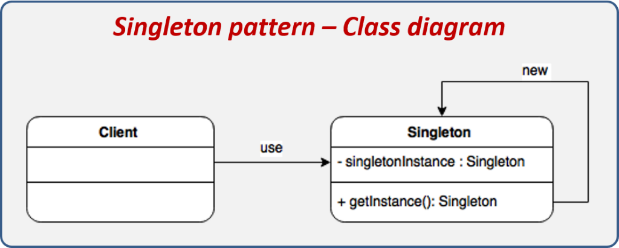
\includegraphics[width=2.81in,height=1.13in]{./media/image7.png}
	\end{Center}
\end{figure}


%%%%%%%%%%%%%%%%%%%% Figure/Image No: 6 Ends here %%%%%%%%%%%%%%%%%%%%

\par

{\fontsize{9pt}{10.8pt}\selectfont \textbf{Participantes:} \par}\par

\begin{itemize}
	\item {\fontsize{9pt}{10.8pt}\selectfont \textbf{Client}: Componente que desea obtener una instancia de la clase Singleton. \par}\par

	\item {\fontsize{9pt}{10.8pt}\selectfont \textbf{Singleton}: Clase que implementa el patrón Singleton, de la cual únicamente se podrá tener una instancia durante toda la vida de la aplicación. \par}
\end{itemize}\par


\vspace{\baselineskip}

\vspace{\baselineskip}

\end{itemize}\section{Patrones Estructurales }

\end{enumerate}
\vspace{\baselineskip}{\fontsize{9pt}{10.8pt}\selectfont Los patrones estructurales se enfocan en como las clases y objetos se componen para formar estructuras mayores, los patrones estructurales describen como las estructuras compuestas por clases crecen para crear nuevas funcionalidades de manera de agregar a la\ estructura flexibilidad y que la misma pueda cambiar en tiempo de ejecución lo cual es imposible con una composición de clases estáticas.  \par}\par


\vspace{\baselineskip}
{\fontsize{9pt}{10.8pt}\selectfont Entre los más conocidos elegimos 3, los cuales son:\par}\par

	\item {\fontsize{9pt}{10.8pt}\selectfont \textbf{Patrón Adapter}\par}\par



%%%%%%%%%%%%%%%%%%%% Figure/Image No: 7 starts here %%%%%%%%%%%%%%%%%%%%

\begin{figure}[H]
	\begin{FlushRight}		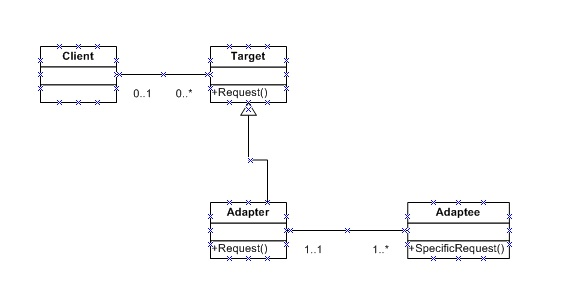
\includegraphics[width=2.81in,height=1.46in]{./media/image8.png}
	\end{FlushRight}\end{figure}


%%%%%%%%%%%%%%%%%%%% Figure/Image No: 7 Ends here %%%%%%%%%%%%%%%%%%%%

{\fontsize{9pt}{10.8pt}\selectfont \textbf{Definición:} Convierte la interfaz de una clase en otra que espera un cliente.\par}\par

{\fontsize{9pt}{10.8pt}\selectfont \textbf{Participantes: }\par}\par


\vspace{\baselineskip}
{\fontsize{9pt}{10.8pt}\selectfont \textbf{Target:} Define la clase que es esperada por el cliente. \par}\par

{\fontsize{9pt}{10.8pt}\selectfont \textbf{Adapter:} Adapta la clase a otra esperada por el cliente. \par}\par

{\fontsize{9pt}{10.8pt}\selectfont \textbf{Adaptee:} Define la clase que necesita a ser adaptada. \par}\par

{\fontsize{9pt}{10.8pt}\selectfont \textbf{Client:} Consume el servicio target. \par}\par


\vspace{\baselineskip}
{\fontsize{9pt}{10.8pt}\selectfont Este patrón se usa comúnmente en los casos en los que queremos utilizar una clase cuya interfaz no coincide con nuestras necesidades.\par}\par


\vspace{\baselineskip}

\vspace{\baselineskip}
	\item {\fontsize{9pt}{10.8pt}\selectfont  \textbf{Patrón Brigde}\par}\par

{\fontsize{9pt}{10.8pt}\selectfont \textbf{Definición:} Desacopla una clase abstracta de su implementación final de manera de que ambas puedan ser independientes.\par}\par



%%%%%%%%%%%%%%%%%%%% Figure/Image No: 8 starts here %%%%%%%%%%%%%%%%%%%%

\begin{figure}[H]
	\begin{Center}
		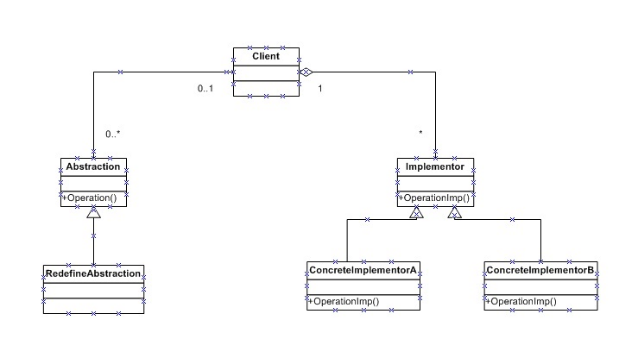
\includegraphics[width=2.81in,height=1.54in]{./media/image9.png}
	\end{Center}
\end{figure}


%%%%%%%%%%%%%%%%%%%% Figure/Image No: 8 Ends here %%%%%%%%%%%%%%%%%%%%

\par

{\fontsize{9pt}{10.8pt}\selectfont \textbf{Participantes: }\par}\par


\vspace{\baselineskip}
{\fontsize{9pt}{10.8pt}\selectfont \textbf{Abstraction:} Define una interfaz abstracta y mantiene una referencia a un objeto del tipo Implementor. \par}\par


\vspace{\baselineskip}
{\fontsize{9pt}{10.8pt}\selectfont \textbf{RefinedAbstraction}: Extiende de la interfaz definida por la clase Abstraction. \par}\par


\vspace{\baselineskip}
{\fontsize{9pt}{10.8pt}\selectfont \textbf{Implementor:} Define la interfaz para la clase que realiza la implementación, la misma no tiene una correspondencia exacta con la interfaz Abstraction, de hecho, ambas interfaces pueden ser completamente diferentes. \par}\par


\vspace{\baselineskip}
{\fontsize{9pt}{10.8pt}\selectfont \textbf{ConcreteImplementor}: Implementa la interfaz Implementor y define una implementación en concreto.\par}\par


\vspace{\baselineskip}

\vspace{\baselineskip}

\vspace{\baselineskip}

\vspace{\baselineskip}
{\fontsize{9pt}{10.8pt}\selectfont $\bullet$ \tab \textbf{ Patrón Composite}\par}\par


\vspace{\baselineskip}
{\fontsize{9pt}{10.8pt}\selectfont \textbf{Definición:} Este patrón construye objetos dentro de una estructura de árbol, de esta manera los objetos que componen el árbol pueden tratarse de manera individual o como una composición de objetos.\par}\par


\vspace{\baselineskip}
{\fontsize{9pt}{10.8pt}\selectfont  \par}\par


\vspace{\baselineskip}
{\fontsize{9pt}{10.8pt}\selectfont Como podemos ver en este patrón los objetos pueden estar compuestos por objetos más complejos que a su vez pueden ser también objetos compuestos y así sucesivamente, sin embargo, un cliente podría manejar una estructura compuesta o una simple de manera uniforme y sin necesidad de saber si están tratando con objetos compuestos o no.\par}\par



%%%%%%%%%%%%%%%%%%%% Figure/Image No: 9 starts here %%%%%%%%%%%%%%%%%%%%

\begin{figure}[H]
	\begin{Center}
		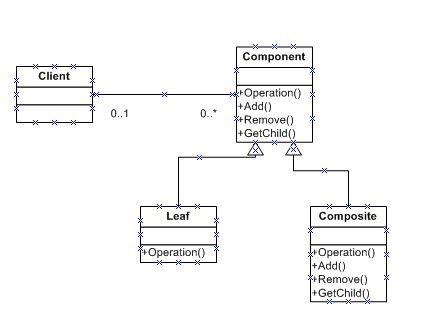
\includegraphics[width=2.81in,height=2.14in]{./media/image10.png}
	\end{Center}
\end{figure}


%%%%%%%%%%%%%%%%%%%% Figure/Image No: 9 Ends here %%%%%%%%%%%%%%%%%%%%

\par


\vspace{\baselineskip}
{\fontsize{9pt}{10.8pt}\selectfont \textbf{Participantes: }\par}\par


\vspace{\baselineskip}
{\fontsize{9pt}{10.8pt}\selectfont \textbf{Component:} Declara una interfaz que implementa los objetos en el árbol, define el comportamiento por defecto de los objetos en el árbol y la manera en la que se acceden y se administran los hijos de la composición. \par}\par


\vspace{\baselineskip}
{\fontsize{9pt}{10.8pt}\selectfont \textbf{Leaf:} Representa una rama de objetos dentro del árbol o composición, una Leaf no tiene hijos y define el comportamiento de objetos primitivos en la composición. \par}\par


\vspace{\baselineskip}
{\fontsize{9pt}{10.8pt}\selectfont \textbf{Composite:} Define el comportamiento para los hijos que posee y almacena los mismos. \par}\par


\vspace{\baselineskip}
{\fontsize{9pt}{10.8pt}\selectfont \textbf{Client}: Manipula los objetos de la composición a través de la interfaz de los componentes. Este patrón permite que un cliente pueda interactuar con los objetos que componen toda una estructura. \par}\par


\vspace{\baselineskip}
{\fontsize{9pt}{10.8pt}\selectfont Como podemos ver en este patrón los objetos pueden estar compuestos por objetos más complejos que a su vez pueden ser también objetos compuestos y así sucesivamente, sin embargo, un cliente podría manejar una estructura compuesta o una simple de manera uniforme y sin necesidad de saber si están tratando con objetos compuestos o no.\par}\par


\vspace{\baselineskip}

\vspace{\baselineskip}
\section{Patrones de comportamientos}
{\fontsize{9pt}{10.8pt}\selectfont Se centran en las formas de como interactúan y como se reparten las responsabilidades las distintas clases y objetos.\par}\par

{\fontsize{9pt}{10.8pt}\selectfont $\bullet$ \tab \textbf{ Patrón Observer}\par}\par

{\fontsize{9pt}{10.8pt}\selectfont \textbf{Definicion: }El patrón de diseño Observer permite observar los cambios producidos por un objeto, de esta forma, cada cambio que afecte el estado del objeto observado lanzará una notificación a los observadores; a esto se le conoce como Publicador-Suscriptor. Observer es uno de los principales patrones de diseño utilizados en interfaces gráficas de usuario (GUI), ya que permite desacoplar al componente gráfico de la acción a realizar. \par}\par



%%%%%%%%%%%%%%%%%%%% Figure/Image No: 10 starts here %%%%%%%%%%%%%%%%%%%%

\begin{figure}[H]
	\begin{Center}
		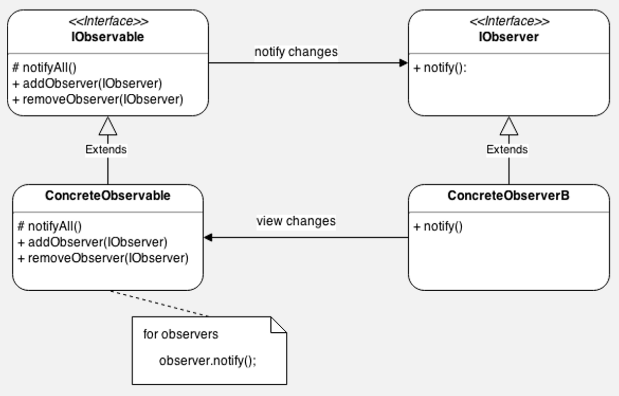
\includegraphics[width=2.81in,height=1.8in]{./media/image11.png}
	\end{Center}
\end{figure}


%%%%%%%%%%%%%%%%%%%% Figure/Image No: 10 Ends here %%%%%%%%%%%%%%%%%%%%

{\fontsize{10pt}{12.0pt}\selectfont \par}\par

{\fontsize{9pt}{10.8pt}\selectfont \textbf{Participantes: }\par}\par

{\fontsize{9pt}{10.8pt}\selectfont \textbf{IObservable:} Interface que deben de implementar todos los objetos que quieren ser observados, en ella se definen los métodos mínimos que se deben implementar. \par}\par

{\fontsize{9pt}{10.8pt}\selectfont \textbf{ConcreteObservable}: Clase que desea ser observada, ésta implementa IObservable y debe implementar sus métodos. \par}\par

{\fontsize{9pt}{10.8pt}\selectfont \textbf{IObserver:} Interfaces que deben implementar todos los objetos que desean observar los cambios de IObservable. \par}\par

{\fontsize{9pt}{10.8pt}\selectfont \textbf{ConcreteObserver:} Clase concreta que está atenta de los cambios de IObserver, esta clase hereda de IObserver y debe de implementar sus métodos. \par}\par

{\fontsize{9pt}{10.8pt}\selectfont  \par}\par


\vspace{\baselineskip}

\vspace{\baselineskip}
{\fontsize{9pt}{10.8pt}\selectfont El patrón de diseño Observer es parecido al patrón Mediator, si bien en él una clase central encapsula y dirige la comunicación generada entre los demás objetos. \par}\par


\vspace{\baselineskip}

\vspace{\baselineskip}

\vspace{\baselineskip}

\vspace{\baselineskip}

\vspace{\baselineskip}

\vspace{\baselineskip}
{\fontsize{10pt}{12.0pt}\selectfont \textbf{Funcionamiento: }\par}\par



%%%%%%%%%%%%%%%%%%%% Figure/Image No: 11 starts here %%%%%%%%%%%%%%%%%%%%

\begin{figure}[H]		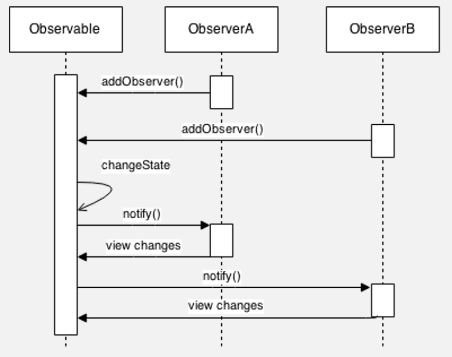
\includegraphics[width=2.81in,height=2.22in]{./media/image12.png}
\end{figure}


%%%%%%%%%%%%%%%%%%%% Figure/Image No: 11 Ends here %%%%%%%%%%%%%%%%%%%%

{\fontsize{10pt}{12.0pt}\selectfont \textbf{ }\par}\par

{\fontsize{10pt}{12.0pt}\selectfont \textbf{ }\par}\par

{\fontsize{10pt}{12.0pt}\selectfont \textbf{ }\par}\par

\begin{enumerate}[label*={\fontsize{9pt}{9pt}\selectfont \arabic*.}]
	\item {\fontsize{9pt}{10.8pt}\selectfont El ObserverA se registra con el objeto Observable para ser notificado de algún cambio. \par}
\end{enumerate}\par

\begin{enumerate}[label*={\fontsize{9pt}{9pt}\selectfont \arabic*.}]
	\item {\fontsize{9pt}{10.8pt}\selectfont El ObserverB se registra con el objeto Observable para ser notificado de algún cambio. \par}
\end{enumerate}\par

\begin{enumerate}[label*={\fontsize{9pt}{9pt}\selectfont \arabic*.}]
	\item {\fontsize{9pt}{10.8pt}\selectfont Ocurre algún cambio en el estado del Observable. \par}
\end{enumerate}\par

\begin{enumerate}[label*={\fontsize{9pt}{9pt}\selectfont \arabic*.}]
	\item {\fontsize{9pt}{10.8pt}\selectfont Todos los Observers son notificados con el cambio ocurrido. \par}
\end{enumerate}\par


\vspace{\baselineskip}
{\fontsize{9pt}{10.8pt}\selectfont $\bullet$ \tab \textbf{ Patrón Vistor}\par}\par

\textbf{ }{\fontsize{9pt}{10.8pt}\selectfont \textbf{Definicion:} El patrón de diseño Visitor se utiliza para separar la lógica u operaciones que se pueden realizar sobre una estructura compleja. En ocasiones nos podemos encontrar con estructuras de datos que requieren realizar operaciones sobre ella, pero estas operaciones pueden ser muy variadas e incluso se pueden desarrollar nuevas a medida que la aplicación crece. \par}\par



%%%%%%%%%%%%%%%%%%%% Figure/Image No: 12 starts here %%%%%%%%%%%%%%%%%%%%

\begin{figure}[H]
	\begin{Center}
		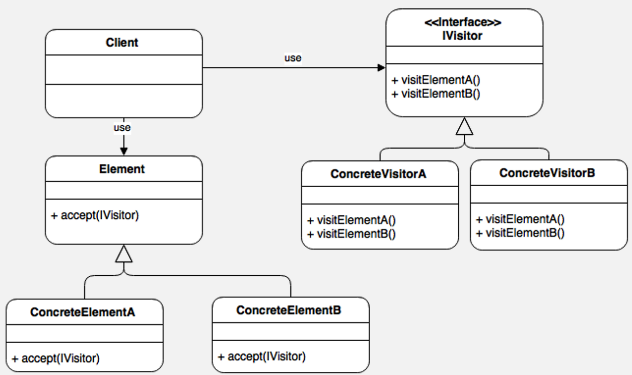
\includegraphics[width=2.81in,height=1.67in]{./media/image13.png}
	\end{Center}
\end{figure}


%%%%%%%%%%%%%%%%%%%% Figure/Image No: 12 Ends here %%%%%%%%%%%%%%%%%%%%

\par


\vspace{\baselineskip}
{\fontsize{9pt}{10.8pt}\selectfont \textbf{Participantes: }\par}\par

{\fontsize{9pt}{10.8pt}\selectfont \textbf{Cliente: }Componente que interactúa con la estructura (element) y con el Visitante, éste es responsable de crear los visitantes y enviarlos al elemento para su procesamiento. \par}\par

{\fontsize{9pt}{10.8pt}\selectfont \textbf{Element: }Representa la raíz de la estructura, en forma de árbol, sobre la que utilizaremos el Visitante. Este objeto por lo general es una interface que define el método accept y deberán implementar todos los objetos de la estructura. \par}\par

{\fontsize{9pt}{10.8pt}\selectfont \textbf{ConcreteElement: }Representa un hijo de la estructura compuesta, la estructura completa puede estar compuesta de un gran número de estos objetos y cada uno deberá implementar el método accept. \par}\par

{\fontsize{9pt}{10.8pt}\selectfont \textbf{IVisitor: }Interface que define la estructura del visitante, la interface deberá tener un método por cada objeto que se requiera analizar de la estructura (element). \par}\par

{\fontsize{9pt}{10.8pt}\selectfont \textbf{ConcreteVisitor: }Representa una implementación del visitante, esta implementación puede realizar una operación sobre el element. Es posible tener todos los ConcreteVisitor necesarios para realizar las operaciones que necesitemos. \par}\par

{\fontsize{9pt}{10.8pt}\selectfont  \par}\par

{\fontsize{9pt}{10.8pt}\selectfont \textbf{Funcionamiento:} \par}\par

{\fontsize{9pt}{10.8pt}\selectfont  \par}\par



%%%%%%%%%%%%%%%%%%%% Figure/Image No: 13 starts here %%%%%%%%%%%%%%%%%%%%

\begin{figure}[H]
	\begin{Center}
		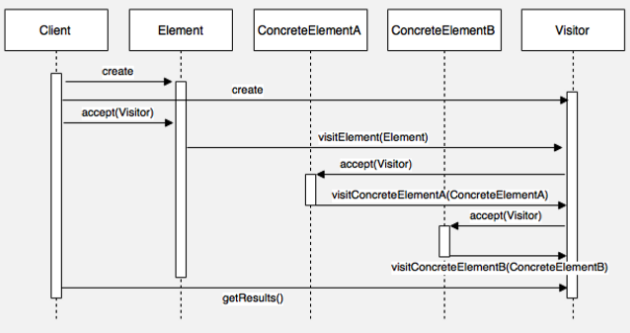
\includegraphics[width=2.81in,height=1.57in]{./media/image14.png}
	\end{Center}
\end{figure}


%%%%%%%%%%%%%%%%%%%% Figure/Image No: 13 Ends here %%%%%%%%%%%%%%%%%%%%

{\fontsize{9pt}{10.8pt}\selectfont  \par}\par

\begin{enumerate}[label*={\fontsize{9pt}{9pt}\selectfont \arabic*.}]
	\item {\fontsize{9pt}{10.8pt}\selectfont El \textit{cliente }crea la estructura (Element). \par}
\end{enumerate}\par

\begin{enumerate}[label*={\fontsize{9pt}{9pt}\selectfont \arabic*.}]
	\item {\fontsize{9pt}{10.8pt}\selectfont El cliente crea la instancia del Visitante a utilizar sobre la estructura. \par}
\end{enumerate}\par

\begin{enumerate}[label*={\fontsize{9pt}{9pt}\selectfont \arabic*.}]
	\item {\fontsize{9pt}{10.8pt}\selectfont El cliente ejecuta el método accept de la estructura y la envía al Visitante. \par}
\end{enumerate}\par

\begin{enumerate}[label*={\fontsize{9pt}{9pt}\selectfont \arabic*.}]
	\item {\fontsize{9pt}{10.8pt}\selectfont El Element le dice al Visitante con que método lo debe procesar. El Visitante deberá tener un método para cada tipo de clase de la estructura. \par}
\end{enumerate}\par

\begin{enumerate}[label*={\fontsize{9pt}{9pt}\selectfont \arabic*.}]
	\item {\fontsize{9pt}{10.8pt}\selectfont El Visitante analiza al Element mediante su método visitElement y repite el proceso de ejecutar el método accept sobre los hijos del Element. Nuevamente el Visitante deberá tener un método para procesar cada clase hija de la estructura. \par}
\end{enumerate}\par

\begin{enumerate}[label*={\fontsize{9pt}{9pt}\selectfont \arabic*.}]
	\item {\fontsize{9pt}{10.8pt}\selectfont El ConcreteElementA le indica al Visitante con qué método debe procesarlo, el cual es visitElementA. \par}
\end{enumerate}\par

\begin{enumerate}[label*={\fontsize{9pt}{9pt}\selectfont \arabic*.}]
	\item {\fontsize{9pt}{10.8pt}\selectfont La visitante continúa con los demás hijos de Element y esta vez ejecuta el método accept sobre el ConcreteElementB. \par}
\end{enumerate}\par

\begin{enumerate}[label*={\fontsize{9pt}{9pt}\selectfont \arabic*.}]
	\item {\fontsize{9pt}{10.8pt}\selectfont El ConcrteElementB le indica al Visitante con qué método debe procesarlo, el cual es visitElementB. \par}
\end{enumerate}\par

\begin{enumerate}[label*={\fontsize{9pt}{9pt}\selectfont \arabic*.}]
	\item {\fontsize{9pt}{10.8pt}\selectfont Finalmente, el Visitante termina la operación sobre la estructura cuando ha recorrido todos los objetos, obteniendo un resultado que es solicitado por el cliente mediante el método getResults (el resultado es opcional ya que existen operaciones que no arrojan resultados). \par}
\end{enumerate}\par


\vspace{\baselineskip}

\vspace{\baselineskip}
{\fontsize{9pt}{10.8pt}\selectfont .\par}\par

\textbf{\ \ \ \  VI. CONCLUCIONES}\par

\begin{itemize}
	\item {\fontsize{9pt}{10.8pt}\selectfont Los patrones de diseño ayudan a estandarizar el código. \par}\par

	\item {\fontsize{9pt}{10.8pt}\selectfont Hacen que el diseño sea más comprensible para otros programadores. \par}\par

	\item {\fontsize{9pt}{10.8pt}\selectfont Estamos mal si pensamos usarlos porque los demás lo hacen. \par}\par

	\item {\fontsize{9pt}{10.8pt}\selectfont Los Patrones de diseño son una solución general para problemas conocidos, pero se adaptan de acuerdo a contextos específicos. \par}\par

	\item {\fontsize{9pt}{10.8pt}\selectfont La mayor complejidad, que representan, es saber cuándo utilizarlos. \par}
\end{itemize}\par


\vspace{\baselineskip}
{\fontsize{9pt}{10.8pt}\selectfont  \par}\par

\section{RECOMENDACIONES}

\vspace{\baselineskip}
\vspace{\baselineskip}
\vspace{\baselineskip}\section{Si no usas patrones, deberías hacerlo. Los patrones ayudan a estandarizar el código, haciendo que el diseño sea más comprensible para otros programadores. Son muy buenas herramientas, y como programadores, siempre deberíamos usar las mejores herramientas a nuestro alcance. }
\section{De nada vale aplicar patrones sin una buena razón. }

\vspace{\baselineskip}
\vspace{\baselineskip}
\vspace{\baselineskip}\section*{VIII. BIBLIOGRAFIA}
\addcontentsline{toc}{section}{VIII. BIBLIOGRAFIA}

\vspace{\baselineskip}
{\fontsize{9pt}{10.8pt}\selectfont 2020). Recuperado 21 Julio 2020, de: http://siul02.si.ehu.es/$ \sim $ alfredo/iso/06Patrones.pdf \par}\par


\vspace{\baselineskip}
{\fontsize{9pt}{10.8pt}\selectfont  \par}\par

{\fontsize{9pt}{10.8pt}\selectfont Los Patrones de Diseño Hoy: Patrones de Comportamiento $ \vert $  Koalite. (2018). Recuperado 21 Julio 2020, de: https://blog.koalite.com/2016/12/los-patrones-de-diseno-hoy-patrones-de-comportamiento/ \par}\par


\vspace{\baselineskip}
{\fontsize{9pt}{10.8pt}\selectfont  \par}\par

{\fontsize{9pt}{10.8pt}\selectfont Observer. (2019). Recuperado 21 Julio 2020, de: https://reactiveprogramming.io/blog/es/patrones-de-diseno/observer \par}\par


\vspace{\baselineskip}
{\fontsize{9pt}{10.8pt}\selectfont  \par}\par


\vspace{\baselineskip}
{\fontsize{9pt}{10.8pt}\selectfont Patrón de diseño Command (comportamiento). (2019). Recuperado 21 Julio 2020, de: https://informaticapc.com/patrones-de-diseno/command.php \par}\par


\vspace{\baselineskip}

\vspace{\baselineskip}
{\fontsize{9pt}{10.8pt}\selectfont Patrón de diseño Command (comportamiento). (2019). Recuperado 21 Julio 2020, de: https://informaticapc.com/patrones-de-diseno/command.php \par}\par


\vspace{\baselineskip}
{\fontsize{9pt}{10.8pt}\selectfont Patrones de diseño creacionales. (2016). Recuperado 21 Julio 2020, de: https://ed.team/blog/patrones-de-diseno-creacionales \par}\par


\vspace{\baselineskip}

\vspace{\baselineskip}
{\fontsize{9pt}{10.8pt}\selectfont Patrones Estructurales. (2019). Recuperado 21 Julio 2020, de: https://highscalability.wordpress.com/2010/04/12/patrones$\%$ C2$\%$ A0estructurales/ \par}\par


\vspace{\baselineskip}
{\fontsize{9pt}{10.8pt}\selectfont  \par}\par


\vspace{\baselineskip}
{\fontsize{9pt}{10.8pt}\selectfont Programacion en Castellano, S. (2018). Patrones de Diseño (XIX): Patrones de Comportamiento - Mediator. Recuperado 21 Julio 2020, de: \par}\par


\vspace{\baselineskip}
{\fontsize{9pt}{10.8pt}\selectfont https://programacion.net/articulo/patrones\_de\_diseno\_xix\_patrones\_de\_comportamiento\_mediator\_1022\par}\par


\vspace{\baselineskip}

\vspace{\baselineskip}
\vspace{\baselineskip}
\setlength{\parskip}{8.04pt}

\vspace{\baselineskip}

\vspace{\baselineskip}

\end{multicols}

\vspace{\baselineskip}

\vspace{\baselineskip}

\vspace{\baselineskip}

\printbibliography
\end{document}